\documentclass[titlepage = firstcover]{scrartcl}
\usepackage[aux]{rerunfilecheck}
\usepackage{fontspec}
\usepackage[main=ngerman, english, french]{babel}

% mehr Pakete hier
\usepackage{expl3}
\usepackage{xparse}

%Mathematik------------------------------------------------------
\usepackage{amsmath}   % unverzichtbare Mathe-Befehle
\usepackage{amssymb}   % viele Mathe-Symbole
\usepackage{mathtools} % Erweiterungen für amsmath
\usepackage[
  math-style=ISO,    % \
  bold-style=ISO,    % |
  sans-style=italic, % | ISO-Standard folgen
  nabla=upright,     % |
  partial=upright,   % /
]{unicode-math}% "Does exactly what it says on the tin."
\usepackage[section, below]{placeins}

% Laden von OTF-Mathefonts
% Ermöglich Unicode Eingabe von Zeichen: α statt \alpha

\setmathfont{Latin Modern Math}
%\setmathfont{Tex Gyre Pagella Math} % alternativ zu Latin Modern Math
\setmathfont{XITS Math}[range={scr, bfscr}]
\setmathfont{XITS Math}[range={cal, bfcal}, StylisticSet=1]

\AtBeginDocument{ % wird bei \begin{document}
  % werden sonst wieder von unicode-math überschrieben
  \RenewDocumentCommand \Re {} {\operatorname{Re}}
  \RenewDocumentCommand \Im {} {\operatorname{Im}}
}
\usepackage{mleftright}
\setlength{\delimitershortfall}{-1sp}

%Sprache----------------------------------------------------------
\usepackage{microtype}
\usepackage{xfrac}
\usepackage[autostyle]{csquotes}    % babel
\usepackage[unicode, pdfusetitle]{hyperref}
\usepackage{bookmark}
\usepackage[shortcuts]{extdash}
%Einstellungen hier, z.B. Fonts
\usepackage{booktabs} % Tabellen


\title{Der Compton-Effekt}
\author{
  Lasse Sternemann\\
  \href{mailto:lasse.sternemann@udo.edu}{lasse.sternemann@udo.edu}
}
\date{Bearbeitet am 01.05.2020}

\begin{document}
    \maketitle
    \newpage
    \tableofcontents
    \newpage

    \section{Theoretische Grundlagen}
        \subsection{Compton-Effekt}
        Wenn ein Photon auf ein freies Elektron trifft, findet ein elastischer Stoß statt. Dabei wird ein Teil des Impulses sowie ein Teil der 
        Energie des Photons an das Elektron übertragen. Aufgrund des Energieverlustes des Photons vergrößert sich dessen Wellenlänge. Dies ist in 
        Gleichung \ref{eqn:EPhoton} zu sehen. Dabei sind das Planck´sche-Wirkungsquantum $h$ und die Lichtgeschwindigkeit $c$ konstant und die Energie $E_{\text{Photon}}$ dementsprehchend
        antiproportional zur Wellenlänge $\lambda$ des Photons ist. 

        \begin{equation}
            E_{\text{Photon}} = \frac{hc}{\lambda}
            \label{eqn:EPhoton}
        \end{equation}
        
        \noindent
        Die Differenz der Wellenlängen des Photons vor $\lambda _1$ und nach dem Stoß $\lambda _2$ lässt sich über die beim elastischen Stoß geltenden
        Impuls- und Energieerhaltung nach Gleichung \ref{eqn:ComptonWellenlänge} berechnen.

        \begin{equation}
            \Delta \lambda = \lambda_1 - \lambda_2 = \frac{h}{c \cdot m_e} \cdot \left(1-\cos(\theta)\right) = \lambda_{\text{C}} \cdot \left(1-\cos(\theta)\right)
            \label{eqn:ComptonWellenlänge}
        \end{equation}
        
        \noindent
        Dabei bezeichnet $\lambda_{\text{C}}$ die Compton-Wellenlänge, die eine Konstante ist. Aus der Gleichung lässt sich erkennen, dass die 
        Wellenlängendifferenz und somit die vom Photon abgegebene Energie vom Streuwinkel $\theta$ \ref{fig:SkizzeCompton} abhängt. Die Wellenlängendifferenz 
        wird für einen Streuwinkel von $\pi$, was einer Reflexion entspricht, maximal. Für einen gegen Null laufenden Streuwinkel geht auch die 
        Wellenlängendifferenz gegen Null und die Compton-Streuung tritt quasi nicht mehr auf.
        \begin{align*}
            \Delta \lambda_{\text{max}} = 2 \cdot \lambda_{\text{C}} \qquad \text{bei} \qquad \theta = \pi \\
            \Delta \lambda_{\text{min}} \longrightarrow 0 \qquad \text{für} \qquad \theta \longrightarrow 0
        \end{align*}
        \noindent

        \FloatBarrier
        \begin{figure}[h]
            \centering
            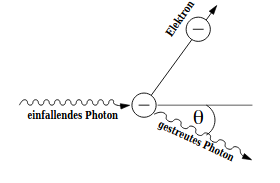
\includegraphics{SkizzeCompton.png}
            \caption{In der Abbildung ist der Compton Effekt skizziert. Der eingezeichnete Winkel $\theta$ ist der Streuwinkel des Photons.[1]}
            \label{fig:SkizzeCompton}
        \end{figure}
        \FloatBarrier
        \noindent

        Dieser Effekt kann bei freien Elektronen für Photonen aller Energien auftreten. Jedoch ist die Wellenlänge sichtbaren Lichts so viel größer
        als die Compton-Wellenlänge (Faktor $10^5$), dass nach der Streuung quasi kein Wellenlängenunterschied zu messen wäre. Zudem tritt der Compton-Effekt
        auch bei in Festkörpern befindlichen Elektronen statt, wenn die Photonenenergie ausreicht, um diese zu lösen. Dies ist bei Röntgen- oder $\gamma$-Strahlung
        der Fall. Die Photonen des sichtbaren Spektrums haben dafür zu wenig Energie.

        \subsection{Röntgenstrahlung}
        Die für den Versuch verwendete Röntgenstrahlung wird in einer Röntgenröhre erzeugt. Dazu werden zunächst Elektronen über eine Heizspannung aus einem
        Glühdraht hinausgelöst und dann durch eine Spannung beschleunigt. Die so beschleunigten Elektronen treffen auf eine Anode und es wird Röntgenstrahlung
        ausgesendet. Das ausgesendete Spektrum setzt sich aus charakteristischen Peaks und einem kontinuierlichen Bremsspektrum zusammen. 
        
            \subsubsection*{Bremsspektrum}
                Das kontinuierliche Bremsspektrum entsteht, wenn die Elektronen sich dem Kern eines Kathodenatoms nähern und dabei durch dessen elektrisches 
                Feld abgebremst werden. Da den Elektronen hierbei eine Beschleunigung widerfährt, verlieren sie ihre kinetische Energie und senden diese als 
                Röntgenphoton aus. Die kleinste Wellenlänge entspricht dabei der Bremsstrahlung der schnellsten Elektronen und hängt von der 
                Beschleunigungsspannung ab.
                
            \subsubsection*{Charakteristische Strahlung}
                Neben der kontinuierlichen Bremsstrahlung entstehen auch Peaks, die vom Anodenmaterial abhängen. Sie entstehen, wenn ein Elektron des Atoms des Anodenmaterials 
                auf ein höheres Energieniveau angeregt wird und dann wieder auf eine niedrigeres Energieniveau zurückspringt. Dabei wird exakt die 
                Energiedifferenz zwischen den beiden Energieniveaus als Röntgenquant abgestrahlt und es entsteht ein Peak im Spektrum.
                
        \subsection{Bragg-Reflexion}
        Um im Experiment die Wellenlänge der Röntgenstrahlung zu bestimmen, wird von der Bragg-Reflexion Gebrauch gemacht. Bei dieser fällt Röntgenstrahlung
        auf ein Material mit Gitterstruktur und wird dabei an den einzelnen Atomen gebeugt. Die Röntgenstrahlung interferiert nun mit sich selbst innerhalb 
        des Gitters. Die zugehörige konstruktive Interferenz findet sich beim Bragg-Winkel $\alpha $ \ref{fig:SkizzeBragg}, der über Formel \ref{eqn:Bragg} 
        mit der Wellenlänge der einfallenden Röntgenstrahlung verknüpft ist. Die notwendige Gitterstruktur ist zum Beispiel in Kristallen gegeben.

        \begin{equation}
            2 \cdot d \cdot \sin(\alpha) = n \cdot \lambda = n \cdot \frac{hc}{E}
            \label{eqn:Bragg}
        \end{equation}

        \noindent
        Der Abstand zwischen den Atomen im Gitter fließt über die Gitterkonstante d \ref{fig:SkizzeBragg} in die Formel ein.
        
        \FloatBarrier
        \begin{figure}[h]
            \centering
            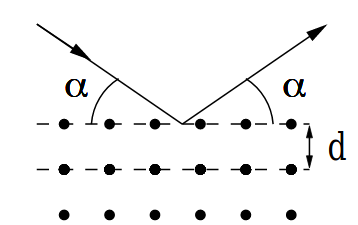
\includegraphics[width = 0.8\linewidth]{Bragg.png}
            \caption{In der Abbildung ist die Bragg-Reflexion skizziert. Der Winkel $\alpha$ ist der Bragg-Winkel und d die Gitterkonstante.[1]}
            \label{fig:SkizzeBragg}
        \end{figure}
        \FloatBarrier

        \subsection{Geiger-Müller-Zählrohr} \label{Geiger}
        Zur Messung der Impulsrate wird ein Geiger-Müller-Zählrohr genutzt. Dieses besteht aus einem mit Gas gefülltem Zylinder, dessen Wand eine große
        Kathode ist. Im Zentrum des Zylinders befindet sich eine Stabanode. Wenn nun ionisierende Strahlung in den Zylinder strahlt, treffen die Photonen
        auf Gasatome und ionisieren diese. Die dabei frei werdenden Elektronen treffen auf den Anodenmantel und werden als einzelner Impuls registriert. Jedes
        ionisierte Gasatom wandert zur Stabanode, um neutral geladen zu werden und so wieder ionisierbar zu sein. Daraus folgt das Problem der Totzeit. Es 
        tritt auf, wenn die Intensität der Strahlung so hoch ist, dass alle Atome ionisiert sind und so nicht die gesamten Impulse gemessen werden. So würde 
        die gemessene Impulsrate trotz kontinuierlich steigender Strahlungsintensität gegen einen Grenzwert laufen. Dieser Effekt wird über die 
        Totzeitkorrektur \ref{eqn:Totzeitkorrektur} behoben. Dabei beschreibt I die korrigierte Impulsrate, N die Impulsrate und $\tau$ die Totzeit.
        
        \begin{equation}
            I = \frac{N}{1-\tau \cdot N}
            \label{eqn:Totzeitkorrektur}
        \end{equation}
        

    \section{Durchführung}
        \subsection{Aufnahme des Röntgenspektrums}
        Um die für den Compton-Effekt notwendige Röntgenstrahlung zu erzeugen, wird eine Kupfer-Röntgenröhre benutzt, die wie bereits beschrieben ein ganzes 
        Spektrum an Röntgenstrahlung aussendet. In diesem Fall verwendet die Röntgenröhre eine Kupferanode zur Röntgenerzeugung und beschleunigt die Elektronen
        fortlaufend mit $35 \, \text{kV}$. Um das Spektrum der 
        erzeugten Röntgenstrahlung darzustellen, wird ein Lithiumfluoridkristall in einem Winkel in den Röntgenstrahl gestellt. Das Geiger-Müller-Zählrohr
        wird im doppelten Winkel des Kristalls zu diesem ausgerichtet. So wird die Bragg-Reflexion ausgenutzt und das Geiger-Müller-Zählrohr misst nur die
        Impulsrate eines speziellen Braggwinkels, dem über Formel \ref{eqn:Bragg} eine Wellenlänge des Röntgenspektrums zugeordnet werden kann. Die Messreihe
        wird in 0,1° Schritten von 8° bis 25° aufgenommen und soll so das gesamte Bremsspektrum sowie die charakteristischen Peaks aufnehmen.
        
        \subsection{Bestimmung der Wellenlängenabhängigkeit der Transmission}
        Für die spätere Bestimmung der Compton-Wellenlänge muss zunächst die Abhängigkeit der Transmission von der Wellenlänge bestimmt werden. Dazu wird dem
        Aufbau zur Aufnahme des Röntgenspektrums ein Aluminium-Absorber hinzugefügt, der zunächst vor der Blende der Röntgenröhre platziert wird. Dann wird 
        wieder der Anstellwinkel des Kristalls zum Röntgenstrahl von 7° bis 10° in 0,1° Schritten variiert und dabei die Impulsrate der bragg-reflektierten
        Strahlung gemessen. Dieselbe Messung wird ohne eingesetzten Aluminium-Absorber wiederholt, um in der Auswertung die Transmission des Aluminium-
        Absorbers zu bestimmen.

        \subsection{Bestimmung der Compton-Wellenlänge}
        Bei der Messung der Impulsrate der compton-gestreuten Photonen werden nur die um 90° gestreuten Photonen gemessen, indem das Geiger-Müller-Zählrohr
        in eben jenen 90° Grad zum Röntgenstrahl platziert wird \ref{fig:SkizzeAbsorber}. 
        Zunächst muss die Grundimpulsrate $I_0$ der compton-gestreuten Photonen aus der Röntgenröhre gemessen werden. Dazu wird ohne Einsatz eines Absorbers
        die an einem Plexiglas gestreute Röntgenstrahlung gemessen. Der Plexiglas-Streuer wird dazu in einem 45° Winkel in dem Röntgenstrahl platziert und es 
        wird eine Impulsrate aufgenommen. Daraufhin wird der Aluminium-Absorber vor die Blende gesetzt \ref{fig:SkizzeAbsorber} und bei restlich gleich bleibendem Aufbau wieder
        eine Impulsrate $I_1$ gemessen. Zuletzt wird der Aluminium-Absorber zwischen das Geiger-Müller-Zählrohr und den Plexiglas-Streuer gesetzt  
        \ref{fig:SkizzeCompton} und wieder bei restlich gleichbleibendem Aufbau eine Impulsrate $I_2$ gemessen.

        \FloatBarrier
        \begin{figure}[h]
            \centering
            \caption{In der Abbildung ist der Aufbau zur Messung der Impulsraten der gestreuten Strahlung zu sehen. Während in Teil a) der Aufbau zur Messung von $I_1$ und in Teil b) der zu $I_2$ dargestellt ist, entspricht der Aufbau zur Messung von $I_0$ beiden gezeigten bei Entfernung des Aluminium-Absorbers.[1]}
            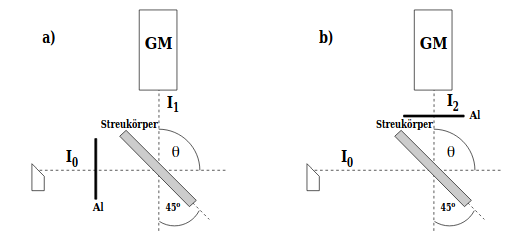
\includegraphics[width = 0.8\linewidth]{absorber.png}
            \label{fig:SkizzeAbsorber}
        \end{figure} 
        \FloatBarrier
        \newpage


    \newpage
    \section{Auswertung}
        %In der gesamten Auswertung werden Ungenauigkeiten von Werten, die von fehlerbehafteten Größen abhängig sind, über die Gauß'sche Fehlerfortpflanzung 
        %für $n$ fehlerbehaftete Größen $x_i$ berechnet.
        %\begin{equation}
        %    \Delta f = \sqrt{\sum_{i=1}^n \left(\frac{\partial f}{\partial x_i} \cdot \Delta x_i\right)}
        %\end{equation}
        %\subsection{Röntgenspektrum}
        Zunächst werden die zur $K_{\alpha}$ und zur $K_{\beta}$ gehörigen Wellenlängen über die literarischen Werte der zugehörigen Energien [2] 
        berechnet, indem Formel \ref{eqn:EPhoton} nach der Wellenlänge umgestellt wird.

        \begin{align}
            \lambda &= \frac{hc}{E_{K_{\alpha, \text{Lit}}}} \approx 160 \,\text{pm} \qquad \text{mit} \, E_{K_{\alpha, \text{Lit}}}=8038 \, \text{eV} \\
            \lambda &= \frac{hc}{E_{K_{\beta, \text{Lit}}}} \approx 140 \,\text{pm} \qquad \text{mit} \, E_{K_{\beta, \text{Lit}}}=8905 \, \text{eV} 
        \end{align}

        \noindent
        Zudem werden die literarischen Bragg-Winkel ausgerechnet, bei denen die zu der $K_{\alpha, \text{Lit}}$ und zur $K_{\beta, \text{Lit}}$ gehörigen Wellenlängen bragg refklektiert werden, 
        sodass die Linien später einfacher im Diagramm identifiziert und verglichen werden können. Dazu wird die Bragg-Bedingung \ref{eqn:Bragg} bei n=1 
        nach $\alpha$ umgestellt. Bei Verwendung eines Lithiumfluoridkristalls beträgt der Netzebenenabstand $d=201,4 \, \text{pm}$ und es ergeben sich
        folgende Winkel:

        \begin{align}
            &\alpha_{K_{\alpha}} = \text{sin}^{-1}\left(\frac{hc}{2d \cdot 8038\cdot eV }\right) \approx 23° \qquad \text{mit} \qquad \lambda = \frac{hc}{E} \\
            &\alpha_{K_{\beta}}  = \text{sin}^{-1}\left(\frac{hc}{2d \cdot 8905\cdot eV }\right) \approx 21°
        \end{align}

        \noindent
        Das experimentell gemessene Spektrum wird in Python über das Matplotlib-Paket dargestellt, indem die Impulsrate gegen den Bragg-Winkel $\alpha$ aufgetragen werden. Die zugehörige 
        Messreihe findet sich im Anhang.
        
        \FloatBarrier
        \begin{figure}[h]
            \centering
            \caption{In der Abbildung ist das Strahlungsspektrum der Kupfer-Röntgenröhre bei 35kV zu sehen. Die Impulsrate wird gegen den Bragg-Winkel aufgetragen, der in Verbindung zur Wellenlänge steht. Neben dem kontinuierlichen Bremsspektrum, das über das gesamte Winkelintervall geht, sind auch die beiden charakteristischen Peaks $K_{\beta}$ bei $(20,2 \pm 0,1)°$ und $K_{\alpha}$ bei $(22,5 \pm 0,1)°$ gut zu erkennen.}
            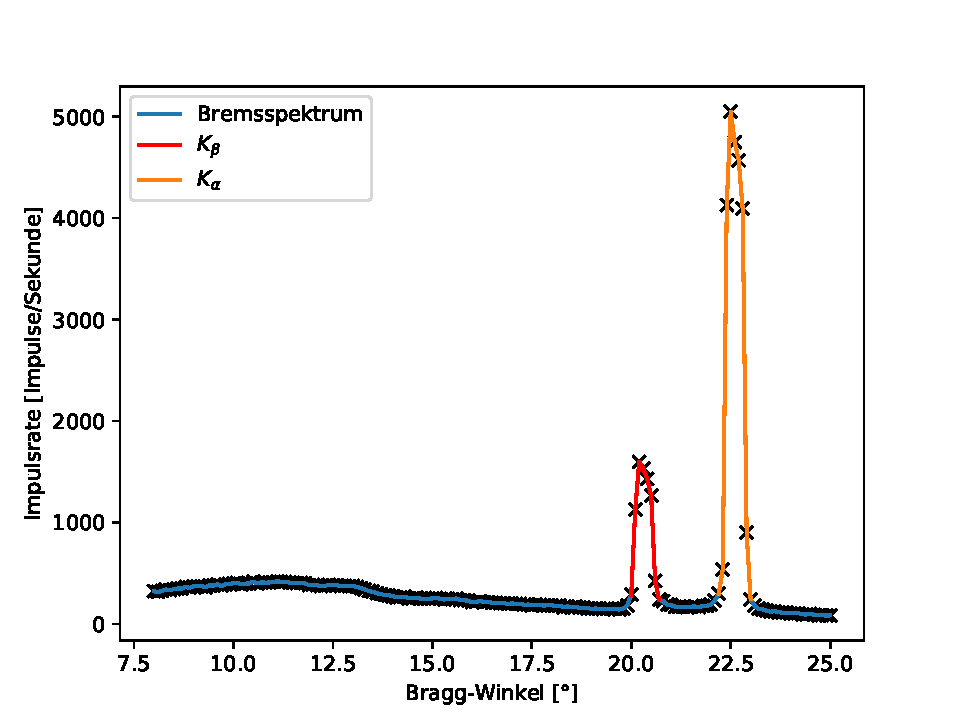
\includegraphics[width = 0.9\linewidth]{Spektrum_Cu.pdf}
            \label{fig:Spektrum}
        \end{figure}
        \FloatBarrier
        \noindent
        Über eine Scipy-Funktion wurden die Maxima der charakteristischen Strahlung wie folgt bestimmt.

        \begin{align}
            &\alpha_{K_{\alpha}} = (22,5 \pm 0,1)°
            &\alpha_{K_{\beta}}  = (20,2° \pm 0,1)°
        \end{align}

        \noindent
        Zum Vergleich mit den Literaturenergien wird diese aus den ermittelten Winkeln über die nach E umgestellte Formel \ref{eqn:Bragg} berechnet.

        \begin{align}
            &E = \frac{hc}{2 \cdot d \cdot \sin(\alpha)} \qquad \text{mit} \qquad d=201,4 \, \text{pm} \nonumber\\
            &E_{K_{\alpha}} = (8043 \pm 34) \, eV \\
            &E_{K_{\beta}}  = (8910 \pm 40) \, eV
            \label{eqn:EGraph}
        \end{align}

        \subsection{Wellenlängenabhängigkeit der Transmission}
        \noindent
        Es wird die Transmission des Aluminiumabsorbers gegen die Wellenlänge aufgetragen. Dazu werden zum einen die Impulsraten $N_1$ und $N_0$ über die 
        Totzeitkorrektur \ref{eqn:Totzeitkorrektur} in die korrigierte Impulsrate und der Winkel über die umgestellte Bragg-Bedingung \ref{eqn:Bragglambda} in die 
        Wellenlänge umgerechnet. Zuletzt wird die Transmission aus dem Quotienten von  $I_1$ und $I_0$ berechnet.

        \begin{equation}
            \lambda = 2dn \cdot \sin(\alpha) \qquad \text{mit} \qquad \text{d}=201,4 \, \text{pm}, \qquad n=1
            \label{eqn:Bragglambda}
        \end{equation}
        \begin{equation}
            T = \frac{I_1}{I_0}
            \label{eqn:Trans}
        \end{equation}
        
        \noindent
        Die gemessenen und korrigierten Werte finden sich im Anhang \ref{tab:Transmission} und werden wieder mit dem Matplotlib-Paket in einem Diagramm aufgetragen. Zudem wird mit der Scipy-Funktion
        Polyfit eine Ausgleichgerade durch die Werte gelegt, die auf folgender Geradengleichung beruht:

        \begin{equation}
            T\left(\lambda \right) = m \cdot \lambda + b\\
            \label{eqn:Regression}
        \end{equation}

        \noindent
        mit folgenden Parametern, deren Abweichung der Covarianzmatrix der linearen Regression entspringt.
        \begin{align}
            m &= (-1,519 \pm 0.024) \cdot 10^{(-10)} \frac{1}{m} \\
            b &= 1.225 \pm 0.014
            \label{eqn:Parameter}
        \end{align}
        \FloatBarrier
        \begin{figure}[h]
            \centering
            \caption{In der Abbildung ist die Wellenlängenabhängigkeit der Transmission des Aluminiumabsorbers zu sehen. Um den linearen Zusammenhang in der Auswertung besser nutzen zu können, wird zudem eine lineare Regression mit angegebenen Parametern \ref{eqn:Regression} über die Messwerte gelegt.}
            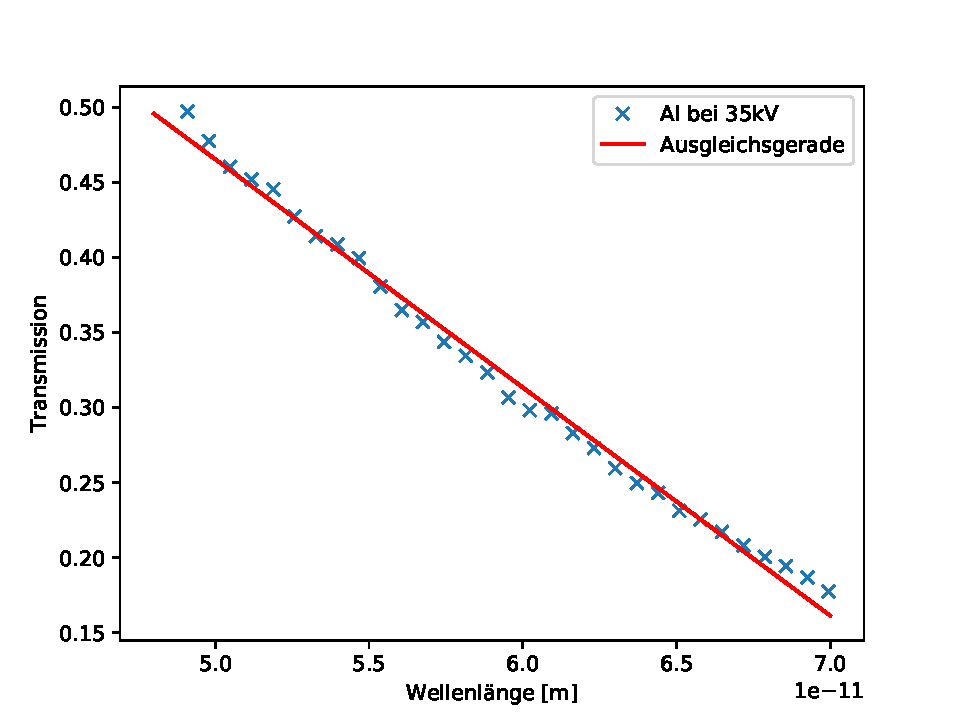
\includegraphics[width = 0.9\linewidth]{Compton_Alu.pdf}
            \label{fig:Transmission}
        \end{figure}
        \FloatBarrier

        \subsection{Bestimmung der Compton-Wellenlänge}
        Mit den bereitstehenden Grundlagen wird die Compton-Wellenlänge bestimmt. Indem die Impulse von nicht gestreuten $I_{\text{ungestreut}}$ 
        und compton-gestreuten $I_{\text{gestreut}}$ Photonen über Formel \ref{eqn:Trans} in die entsprechende Transmission des Aluminiumabsorbers umgerechnet
        werden. Dabei bezeichnet $I_{\text{norm}}$ die Impulse bei gleichem Streuwinkel ohne Aluminiumabsorber. Da die Anzahl der Impulse poisson-verteilt 
        ist, kann der entsprechende Fehler über die Wurzel des Wertes berechnet werden.

        \begin{equation*}
            \Delta I = \sqrt{I}
        \end{equation*}

        \begin{align*}
            I_{\text{norm}} = (2730 \pm 50) \, \text{Impulse}\\
            I_{\text{ungestreut}} = (1180 \pm 34) \, \text{Impulse}\\
            I_{\text{gestreut}} = (1024 \pm 32) \, \text{Impulse}
        \end{align*}
        
        \begin{align}
            T_{\text{ungestreut}} = \frac{I_{\text{ungestreut}}}{I_{\text{norm}}}=0,432 \pm 0,015 \nonumber\\
            T_{\text{gestreut}} = \frac{I_{\text{gestreut}}}{I_{\text{norm}}}=0,375 \pm 0,014 
            \label{eqn:T1T2}
        \end{align}

        \noindent
        Der zugehörige Fehler ergibt sich nach der Gauß'schen Fehlerfortpflanzung wie folgt:     
        \begin{equation*}
            \Delta T = \sqrt{\left( \frac{\Delta I}{I_{\text{norm}}}\right)^2 + \left(\frac{I \cdot \Delta I_{\text{norm}}}{I_{\text{norm}}^2}\right)^2}
        \end{equation*}
        \noindent
        Die den Transmissionen zugehörigen Wellenlängen werden durch Umstellen von \ref{eqn:Regression} nach $\lambda$ und Einsetzen von $T_{\text{ungestreut}}$
        und $T_{\text{gestreut}}$ \ref{eqn:T1T2} ermittelt. Auch deren Fehler ergibt sich aus der Gauß'schen Fehlerfortpflanzung.

        \begin{align}
            \Delta \lambda &= \sqrt{\left(\frac{\Delta T}{m}\right)^2 + \left(\frac{\Delta b}{m}\right)^2 + \left(-\frac{T-b}{m^2} \cdot \Delta m\right)^2} \nonumber \\
            \lambda &= \frac{T - 1,22}{-15\cdot 10^{\left(-9\right)}} \, m \\
            \lambda_{\text{ungestreut}} &= (52,2 \pm 1,6) \, \text{pm} \nonumber \\
            \lambda_{\text{gestreut}} &= (55,9 \pm 1,6)  \, \text{pm} \nonumber
            \label{eqn:y1,y2}
        \end{align}

        \noindent
        Da der Streuwinkkel bei dem Messaufbau 90° beträgt, entspricht die Compton-Wellenlänge $\lambda_{\text{C}}$ der Differenz von $\lambda_{\text{gestreut}}$
        und $\lambda_{\text{ungestreut}}$.
        
        \begin{equation*}
            \Delta \lambda = \lambda_{\text{gestreut}} - \lambda_{\text{ungestreut}} = \lambda_{\text{c}} \cdot \left(1 -\cos (\theta)\right) \\
            \label{eqn:ycexp}
        \end{equation*}

        \begin{equation}
            \lambda_{\text{c}} = \lambda_{\text{gestreut}} - \lambda_{\text{ungestreut}} = (3,8 \pm 1,1) \, \text{pm} \qquad \text{mit} \qquad \theta=90° \\
            \label{eqn:ycwert}
        \end{equation} 



    \section{Diskussion}
        Zunächst ist die Aufnahme des Röntgenspektrums der Kupfer-Röntgenröhre als gelungen zu bezeichnen. Im Spektrum ist die kontinuierliche Bremsstrahlung 
        klar neben den charakteristischen Peaks zu erkennen. Die Energien der gemessenen Peaks \ref{eqn:EGraph} weichen zudem nur geringfügig von den Literaturwerten [2] ab, 
        die $K_{\alpha}\text{-Energie}$ um 0,07 \% , die $K_{\beta}\text{-Energie}$ um 0,1 \%. Der ihnen zugehörige Literaturwert liegt jeweils im Fehlerbereich der Messgröße.
        Die anschließende Bestimmung der Compton-Wellenlänge ergibt eine Wellenlänge (\ref{eqn:ycwert}), die um 43\% von dem Literaturwert [3] abweicht. Der Literaturwert liegt zudem nicht
        im Fehlerbalken der Messgröße. Dieser Fehler ist vermutlich auf den Absorber zurückzuführen. Denn zur genauen Bestimmung der Wellenlänge muss die Absorberdicke vor und nach Streuer gleich sein.
        Dies ist nicht der Fall, wenn die Absorberplatte keine homogene Dicke besitzt und der Punkt der Platte, auf den die Strahlung trifft, bei beiden Positionen nicht derselbe ist. Die Dicke ändert
        sich auch, wenn die Absorberplatte in den beiden Positionen nicht im gleichen Winkel zum Strahl steht. Andererseits könnte die Ungenauigkeit auch auf eine ungenaue Bestimmung der Transmission 
        in Abhängigkeit von der Wellenlänge zurückgeführt werden. Jedoch wurde bei dieser Messung die Totzeitkorrektur durchgeführt und es ergab sich auch ein deutlicher linearer Zusammenhang. 
        Die Frage, ob bei der Messung zur Bestimmung der Compton-Wellenlänge eine Totzeitkorrektur hätte durchgeführt werden müssen, kann mit nein beantwortet werden. Dies ist damit zu begründen,
        dass im gewählten Messbereich von 7° bis 10° nur kleine Zählraten auftreten und die Totzeitkorrektur nur für hohe Zählraten notwendig ist \ref{Geiger}. Letztendlich ist der Fehler 
        vermutlich darauf zurückzuführen, dass die hochenergetische Röntgenstrahlung auch am Aluminiumabsorber compton-streut und dabei womöglich Photonen
        in das Geiger-Müller-Zählrohr gestreut werden.

        \begin{table}[h]
            \centering
            \caption{In der Tabelle werden die Messwerte mit den Literaturwerten verglichen.}
            
            \begin{tabular}{c c c }
                \toprule
                {Messgröße} & {Messwert} & {Literaturwert} \\
                \midrule
                $E_{K_{\alpha}}$ [eV]& 8043$\pm$34 & 8038 \\
                $E_{K_{\beta}}$  [eV]& 8910$\pm$40 & 8905 \\
                $\lambda_C$      [pm}& 3,8$\pm$1,1 & 2,43 \\
                \bottomrule
            \end{tabular}
        \end{table}

    \newpage
    \section{Literaturverzeichnis}
            [1] \textit{Versuchsanleitung V603 - Compton-Effekt.} TU Dortmund, 2020 \newline
            [2] PHYWE Systeme GmbH \& Co. KG: \textit{Charakteristische Röntgenstrahlung von Kupfer} 03.Mai.2020
                \url{http://www.phywe-ru.com/index.php/fuseaction/download/lrn_file/versuchsanleitungen/P2540101/d/p2540101d.pdf} \newline
            [3] National Institute of Standards and Technology: \textit{Fundamental Physical Constants} 03.Mai.2020
                \url{https://physics.nist.gov/cgi-bin/cuu/Value?r}

    \newpage
    

    \begin{table}[h]
        \centering
        \caption{In der Tabelle sind zum einen die primären Messdaten wie der Bragg-Winkel und die zugehörigen Zählraten mit $N_1$ und ohne Aluminiumabsorber $N_2$. Zusätzlich sind auch die daraus berechneten Größen aufgelistet. Die Wellenlänge wird aus dem Bragg-Winkel berechnet \ref{eqn:Bragglambda}, die korrigierten Impulsraten $I_0$ und $I_1$ aus den Impulsraten \ref{eqn:Totzeitkorrektur} und die Transmission T wiederum aus eben diesen korrigierten Impulsraten \ref{eqn:Trans}.}
        \label{tab:Transmission}

        \begin{tabular}{c c c c c c c}
            \toprule
            {$\theta$ [°]}  & {$\lambda$ [pm]} & {$N_0$ [Imp/s]} & {$I_0$ [Imp/s]} & {$N_1$ [Imp/s]} & {$I_1$ [Imp/s]} & {T} \\ 
            \midrule
            7,0$\pm$ 0,1                &  49,1$\pm$ 7,0              &  226,0          &    230,7       &    113,5        &    114,7       &  0,50 \\
            7,1$\pm$ 0,1                &  49,8$\pm$ 7,0              &  232,0          &    237,0       &    112,0        &    113,1       &  0,48 \\
            7,2$\pm$ 0,1                &  50,5$\pm$ 7,0              &  240,5          &    245,8       &    112,0        &    113,1       &  0,46 \\
            7,3$\pm$ 0,1                &  51,2$\pm$ 7,0              &  248,0          &    253,7       &    113,5        &    114,7       &  0,45 \\
            7,4$\pm$ 0,1                &  51,9$\pm$ 7,0              &  255,0          &    261,0       &    115,0        &    116,2       &  0,45 \\
            7,5$\pm$ 0,1                &  52,6$\pm$ 7,0              &  262,0          &    268,3       &    113,5        &    114,7       &  0,43 \\
            7,6$\pm$ 0,1                &  53,3$\pm$ 7,0              &  269,0          &    275,7       &    113,0        &    114,2       &  0,41 \\
            7,7$\pm$ 0,1                &  54,0$\pm$ 7,0              &  276,0          &    283,0       &    114,5        &    115,7       &  0,41 \\
            7,8$\pm$ 0,1                &  54,7$\pm$ 7,0              &  281,0          &    288,3       &    114,0        &    115,2       &  0,40 \\
            7,9$\pm$ 0,1                &  55,4$\pm$ 7,0              &  289,5          &    297,2       &    112,0        &    113,1       &  0,38 \\
            8,0$\pm$ 0,1                &  56,1$\pm$ 7,0              &  295,0          &    303,0       &    109,5        &    110,6       &  0,36 \\
            8,1$\pm$ 0,1                &  56,8$\pm$ 7,0              &  300,0          &    308,3       &    109,0        &    110,1       &  0,36 \\
            8,2$\pm$ 0,1                &  57,5$\pm$ 7,0              &  308,5          &    317,3       &    108,0        &    109,1       &  0,34 \\
            8,3$\pm$ 0,1                &  58,2$\pm$ 7,0              &  311,0          &    320,0       &    106,0        &    107,0       &  0,33 \\
            8,4$\pm$ 0,1                &  58,9$\pm$ 7,0              &  317,0          &    326,3       &    104,5        &    105,5       &  0,32 \\
            8,5$\pm$ 0,1                &  59,6$\pm$ 7,0              &  324,0          &    333,7       &    101,5        &    102,4       &  0,31 \\
            8,6$\pm$ 0,1                &  60,3$\pm$ 7,0              &  328,5          &    338,5       &    100,0        &    101,0       &  0,30 \\
            8,7$\pm$ 0,1                &  61,0$\pm$ 7,0              &  332,5          &    342,8       &    100,5        &    101,4       &  0,30 \\
            8,8$\pm$ 0,1                &  61,7$\pm$ 7,0              &  337,0          &    347,5       &    97,5         &    98,4        &  0,28 \\
            8,9$\pm$ 0,1                &  62,4$\pm$ 7,0              &  340,5          &    351,3       &    95,0         &    95,8        &  0,27 \\
            9,0$\pm$ 0,1                &  63,1$\pm$ 7,0              &  348,0          &    359,3       &    92,5         &    93,3        &  0,26 \\
            9,1$\pm$ 0,1                &  63,7$\pm$ 7,0              &  350,0          &    361,4       &    98,5         &    90,2        &  0,25 \\
            9,2$\pm$ 0,1                &  64,4$\pm$ 7,0              &  353,0          &    364,6       &    88,0         &    88,7        &  0,24 \\
            9,3$\pm$ 0,1                &  65,1$\pm$ 7,0              &  356,5          &    368,3       &    84,5         &    85,1        &  0,23 \\
            9,4$\pm$ 0,1                &  65,8$\pm$ 7,0              &  359,0          &    371,0       &    83,0         &    83,6        &  0,23 \\
            9,5$\pm$ 0,1                &  66,5$\pm$ 7,0              &  363,5          &    375,8       &    81,0         &    81,6        &  0,22 \\
            9,6$\pm$ 0,1                &  67,2$\pm$ 7,0              &  367,0          &    379,5       &    78,5         &    79,1        &  0,21 \\
            9,7$\pm$ 0,1                &  67,9$\pm$ 7,0              &  369,0          &    381,7       &    76,0         &    76,5        &  0,20 \\
            9,8$\pm$ 0,1                &  68,6$\pm$ 7,0              &  370,5          &    383,3       &    74,0         &    74,5        &  0,19 \\
            9,9$\pm$ 0,1                &  69,3$\pm$ 7,0              &  375,0          &    388,1       &    72,0         &    72,5        &  0,19 \\
            10,0$\pm$ 0,1               &  70,0$\pm$ 7,0              &  375,5          &    388,6       &    68,5         &    68,9        &  0,18 \\
            \bottomrule
            
        \end{tabular}
        
    \end{table}

\end{document}